\section{Metodología de trabajo e implementación}
En esta sección en primer lugar hablamos sobre la metodología de trabajo que utilizamos durante todo el proyecto. En segundo lugar describimos las tecnologías utilizadas para el desarrollo de cada una de las partes de la aplicación: el \textit{front-end} (interfaz de usuario), el \textit{back-end} (lógica del negocio e interacción con la base de datos) y la base de datos. Finalmente describimos las arquitecturas que utilizamos.

\subsection{Metodología de trabajo}
Decidimos darle al desarrollo un enfoque ágil\cite{Shore}. Así dar visibilidad constante a todos los interesados fue uno de los principios transversales a todo el proyecto. La comunicación fue muy fluida, tanto por mail, como a través de reuniones presenciales o virtuales (en forma remota). Otro de los pilares del enfoque ágil fue trabajar en forma iterativa e incremental. Es decir que trabajamos con iteraciones de tiempo fijo de una semana de duración. Al final de cada iteración los avances eran validados por el Dr. Reggiani.

\subsubsection{Resumen del itinerario del proyecto}
Lo primero que hicimos fue varias reuniones entre todos los interesados en el proyecto: los desarrolladores, los directores y el Dr. Reggiani. De esas reuniones y de una visita al hospital obtuvimos los requerimientos.

El segundo paso fue la elección de las tecnologías. Entre el basto abanico de posibilidades NodeJS\footnote{http://nodejs.org/} y Grails\footnote{https://grails.org/} aparecían como las predilectas ya que son tecnologías modernas y teníamos buenas referencias de ambas. Para decidirnos por una de las dos desarrollamos un conversor web muy simple de Farenheit a Celcius. A partir de esa primer experiencia finalmente optamos por usar Grails ya que se asemeja más que NodeJS a las tecnologías que veníamos utilizando en las distintas materias a lo largo de la carrera.

Si bien Grails es \textit{full stack}\footnote{Se dice que una tecnología es \textit{full stack} cuando posee todas las herramientas necesarias para desarrollar una aplicación}, decidimos utilizar una tecnología que resuelva las vistas del lado del cliente, se comunique con el \textit{back-end} mediante una interfaz REST\footnote{http://es.wikipedia.org/wiki/Representational\_State\_Transfer} 
y sea \textit{responsive}\footnote{http://es.wikipedia.org/wiki/Diseño\_web\_adaptable}. Así surgió la idea de utilizar AngularJS\footnote{https://angularjs.org/} que cubre ampliamente todos esos requisitos.

En tercer lugar hicimos una estimación relativa a grandes rasgos. Allí calculamos cuanto tiempo nos iba a demandar cada funcionalidad requerida y la fecha de cierre del proyecto. Luego hicimos una planificación en donde ordenamos los requerimientos dentro de las iteraciones según las prioridades del Dr. Reggiani.

\begin{figure}[h]
  \centerline{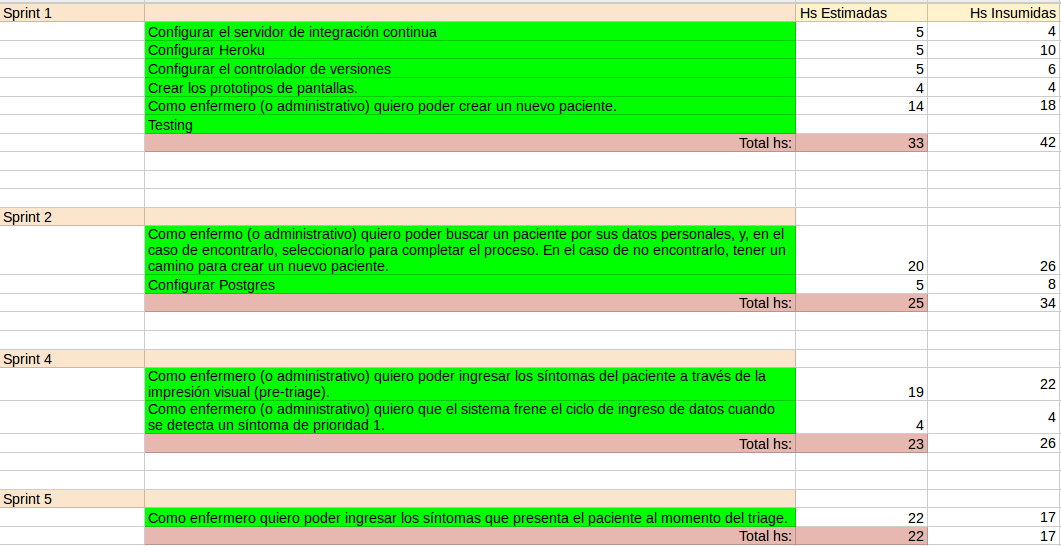
\includegraphics[width=1.2\textwidth]{planificacion.png}}
  \caption{Planificación}
\end{figure}

A partir de ahí comenzamos con el desarrollo recorriendo las iteraciones planificadas. Al promediar el proyecto hicimos una instalación de prueba en el hospital. Y al finalizar el mismo hicimos la instalación definitiva del producto terminado en una máquina de dicha institución.

\subsubsection{Flujo de trabajo en una iteración}
Al inicio de cada iteración estimabamos cuanto tiempo nos iba a llevar cada tarea y enviabamos un email con los detalles sobre lo que ibamos a hacer durante esa semana. También haciamos prototipos de las pantallas a realizar que eran validados por el Dr. Reggiani. Además dejamos sentado en una hoja de cálculo los detalles de cada tarea: el tiempo de realización estimado, la fecha de realización y el tiempo real insumido. Por otro lado cada día que avanzabamos con alguna tarea enviabamos un reporte por email informando lo que habíamos hecho y si había surgido algún contratiempo. Por último, al finalizar la iteración, enviabamos otro email con los detalles de lo realizado.

\begin{figure}[h]
  \centerline{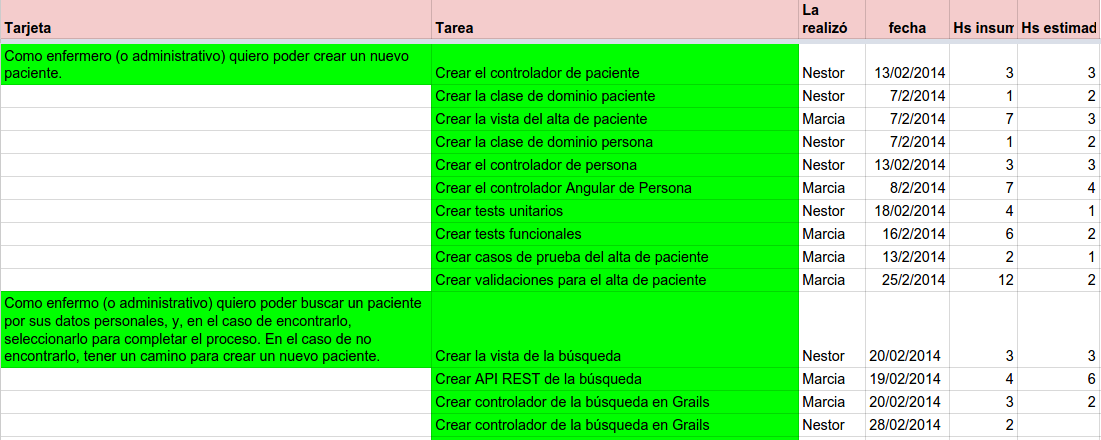
\includegraphics[width=1.2\textwidth]{tracking.png}}
  \caption{\textit{Tracking} de tareas}
\end{figure}

\subsubsection{Herramientas que utilizamos}
Para la comunicación via email creamos un grupo en Google Groups\footnote{https://groups.google.com}.
Para toda la documentación compartida utilizamos Google Drive\footnote{https://drive.google.com/}. Para hacer reuniones remotas utilizamos Skype\footnote{http://www.skype.com.ar/es/} y Google Hangouts\footnote{https://plus.google.com/hangouts}. Utilizamos Balsamiq\footnote{https://balsamiq.com/} para hacer los prototipos de pantallas. Utilizamos Git\footnote{http://git-scm.com/} y Github\footnote{https://github.com/} para versionar el código. Y utilizamos Travis\footnote{https://travis-ci.org/} como servidor de integración continua\footnote{http://es.wikipedia.org/wiki/Integración\_continua}.

\subsection{Tecnologías}
Todas las tecnologías que utilizamos en el desarrollo de la aplicación son de código abierto. Para desarrollar el \textit{front-end} elegimos AngularJS\footnote{https://angularjs.org/}. Para el \textit{back-end} elegimos Grails\footnote{https://grails.org/}.

Cabe aclarar que ambos frameworks cubrieron ampliamente todo lo que nosotros necesitábamos de ellos para hacer este trabajo, por ello sólo utilizamos una pequeña parte de los mismos. Por ejemplo, de Grails casi no utilizamos la parte de las vistas ya que las mismas las desarrollamos del lado del cliente en AngularJS.

Además de estas dos tecnologías utilizamos Bootstrap\footnote{http://getbootstrap.com/} para obtener un diseño amigable para el usuario. Este framework también nos permitió realizar una aplicación \textit{responsive} que se adapta a cualquier tamaño de pantalla, incluso de teléfonos celulares.

\subsubsection{Sobre el \textit{front-end}}
AngularJS es un framework de aplicaciones web de código abierto escrito en JavaScript. Es desarrollado y mantenido por Google. La primer versión fue lanzada en el año 2010 y desde ese momento viene ganando espacio en la industria.

AngularJS es un conjunto de herramientas para la creación de aplicaciones web de una sola página (\textit{single-page applications}). Este framework maneja contenido dinámico y permite extender el vocabulario HTML\footnote{http://es.wikipedia.org/wiki/HTML} obteniendo un entorno más expresivo, legible y práctico para el programador. La filosofía de AngularJS es que la programación declarativa es la que debe utilizarse para generar interfaces de usuario.

\subsubsection{Sobre el \textit{back-end}}
Grails es un framework de aplicaciones web de código abierto para la máquina virtual de Java (JVM). Es un framework \textit{full stack}, es decir que integra todas las herramientas necesarias para desarrollar una aplicación web.

Está escrito en Groovy, un lenguaje de programación que a su vez está desarrollado en Java. Uno de sus principios es la convención sobre la configuración que busca decrementar el número de decisiones que un desarrollador necesita tomar, ganando así en simplicidad pero no perdiendo flexibilidad por ello. La primer versión fue lanzada en el año 2006.

Como está desarrollado en Java, Grails es multiplataforma. Además toma de su lenguaje padre tecnologías ampliamente utilizadas en la industria como Hibernate\footnote{http://es.wikipedia.org/wiki/Hibernate}, para la persistencia de datos, y Spring\footnote{http://es.wikipedia.org/wiki/Spring\_Framework}, para la seguridad, la autenticación, las pruebas, la gestión de transacciones, etc.

\subsubsection{Sobre la base de datos}
Para desarrollar una aplicación como la requerida se hizo indispensable utilizar una base de datos para almacenar toda la información ingresada. Los pacientes, los síntomas, las prioridades, los tiempos de espera, etc. son almacenados en una base de datos.

Durante todo el desarrollo de la aplicación utilizamos una base de datos H2\footnote{http://www.h2database.com} que viene embebida en Grails especialmente para utilizar en la etapa de desarrollo. También utilizamos esa tecnología en la instalación de prueba en el hospital. Pero para la instalación definitiva no utilizamos H2 ya que consideramos más apropiado y seguro tener una base de datos independiente al resto del sistema. Por eso utilizamos PostgreSQL\footnote{http://www.postgresql.org.es/}. PostgreSQL es un sistema de gestión de bases de datos relacional orientado a objetos. Lo elegimos porque varios artículos lo recomiendan como la mejor opción para usar junto a Grails\footnote{https://devcenter.heroku.com/articles/getting-started-with-grails}.


\subsection{Arquitectura}
Utilizamos una arquitectura cliente-servidor\footnote{http://es.wikipedia.org/wiki/Cliente-servidor} con AngularJS del lado del cliente y Grails del lado del servidor.

\subsubsection{Comunicación entre el cliente y el servidor}
La comunicación se da mediante peticiones HTTP\footnote{http://es.wikipedia.org/wiki/Hypertext\_Transfer\_Protocol} desde el cliente (AngularJS) al servidor (Grails). La información viaja en formato JSON\footnote{http://es.wikipedia.org/wiki/JSON}. Ejemplo de petición HTTP desde AngularJS:

\begin{verbatim}
$http.post('usuario/login',{
  usuario: $scope.nombre,
  password: $scope.password
}).success(function(usuario){
  //hago algo cuando la peticion fue exitosa
}).error(function(){
  //hago algo cuando la peticion falló
});		
\end{verbatim}

En este ejemplo, se hace una petición HTTP de tipo POST con un JSON como parámetro. Del lado de Grails quien recibe la petición es el controlador de la clase de dominio Usuario que ejecutara el método login.

\subsubsection{Arquitectura del \textit{front-end}}
En AngularJS cada pantalla esta definida dentro de un archivo HTML. A cada HTML le corresponde un controlador. Todos los controladores están definidos en un módulo de AngularJS dentro de un archivo JavaScript.

Al ser una aplicación de una sóla página, hay un único HTML principal que va cambiando parte de su contenido de manera dinámica a medida que el usuario navega. De esta manera también hay partes de la aplicación que están presentes en todas las pantallas, como el menú principal y el pie de página.

\subsubsection{Arquitectura del \textit{back-end}}
Grails está dividido en vistas, controladores y clases del dominio. Como se trata de una aplicación de una sola página entonces tenemos una única vista. Hay un controlador por cada clase de dominio. Los controladores son los que procesan y responden las peticiones HTTP. Las clases del dominio son las que interactúan con los controladores y la base de datos.

\begin{figure}[h]
\centerline{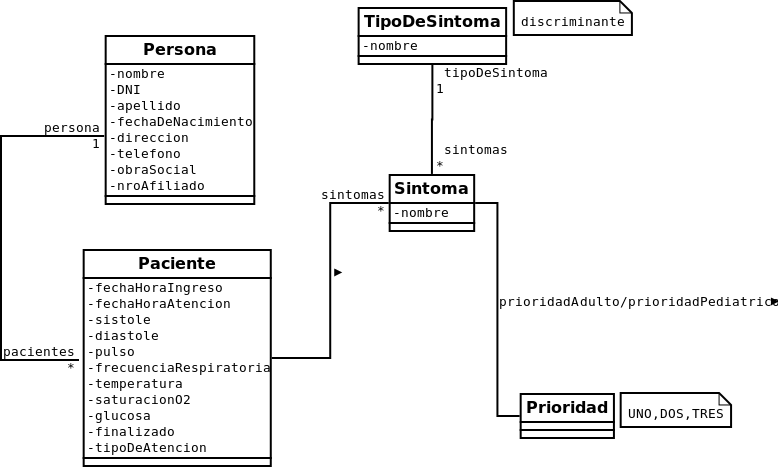
\includegraphics[width=1.2\textwidth]{triage.png}}
\caption{Diagrama de clases del dominio}
\end{figure}